\chapter{Izračun}\label{sec:izracun}

Za izračun ocene parametrov pretočne hidroelektrarne je ključnega pomena pravilen izračun konsumpcijske krivulje za izbran vodotok, saj se vsi nadaljnji izračuni nanašajo nanj. V tem poglavju bom s primerom dokazal, da program računa parametre pravilno. Za dokaz bom uporabil namišljen primer trapezno oblikovane struge vodotoka prikazane na sliki~\ref{fig:izracun_trapeznaStruga}, z 1\% naklonom struge, višino vode v strugi $h=5m$ in Manningovim koeficientom hrapavosti 0,3.

 Rezultate ročnega izračuna bom primerjal z rezultati ki jih izračuna program po trapezni in numerični metodi opisani v poglavju~\ref{sec:teorija_trapeznaMetoda}  oz.~\ref{sec:pretokNumericnaMetoda}. Vse mere na spodnji  sliki~\ref{fig:izracun_trapeznaStruga} so v metrih.



\begin{figure}[ht!]
	\begin{centering}
		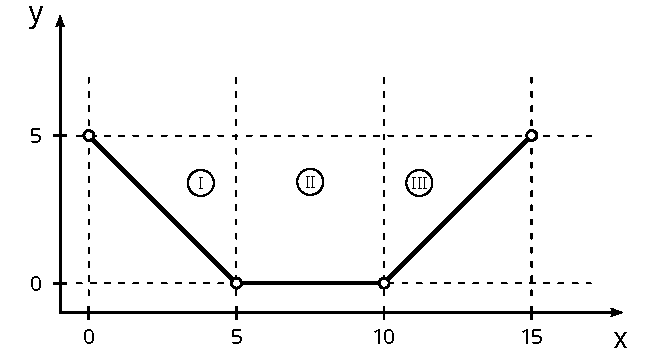
\includegraphics{slike/izracuni/shema_trapezneStruge.pdf}		
		\caption{Shema struge izbranega vodotoka}\label{fig:izracun_trapeznaStruga}
	\end{centering}
\end{figure}




%----------------------------------------------
\section{Izračun parametrov po trapezni metodi}\label{sec:izracun_trapeznaMetoda}



\subsection{Ročni izračun}
Za izračun pretoka vodotoka pri višini $h=5m$ uporabimo enačbe navedene v poglavju~\ref{sec:teorija_trapeznaMetoda}.

\begin{ceqn}
\begin{align}
 P(h)&= b + 2 \cdot \sqrt{h^2 + \left(\dfrac{h} {\tan\alpha} \right)^{2}} = 5 + 2 \cdot \sqrt{5^2 + \left(\dfrac{5} {\tan 45} \right)^{2}} = 19,1~m \\
 S(h)&= b \cdot h +  \dfrac{h^{2}}{\cdot\tan{\alpha}}   = 5  5 +  \dfrac{5^{2}}{\tan{45}}= 50~m^2 \\
 Q(h)&= \dfrac{\sqrt{0,01}}{0,03} \cdot \dfrac{50^{5/3}}{19,1^{2/3}} = 316,6~m^3/s
\end{align}
\end{ceqn}




\subsection{Izračun s programom}
V program vnesemo podatke o rečnem koritu kot je prikazano na sliki~\ref{fig:trapeznaMetoda_vnosPodatkov}.

\begin{figure}[ht!]
	\begin{centering}
		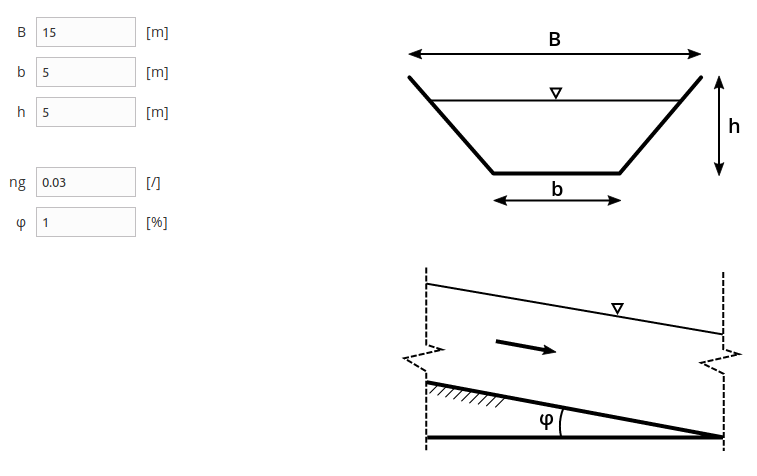
\includegraphics[width=\textwidth]{slike/izracuni/trapeznaStruga.png}		
		\caption{Vnos podatkov v program}\label{fig:trapeznaMetoda_vnosPodatkov}
	\end{centering}
\end{figure}


\begin{figure}[H]
	\begin{centering}
		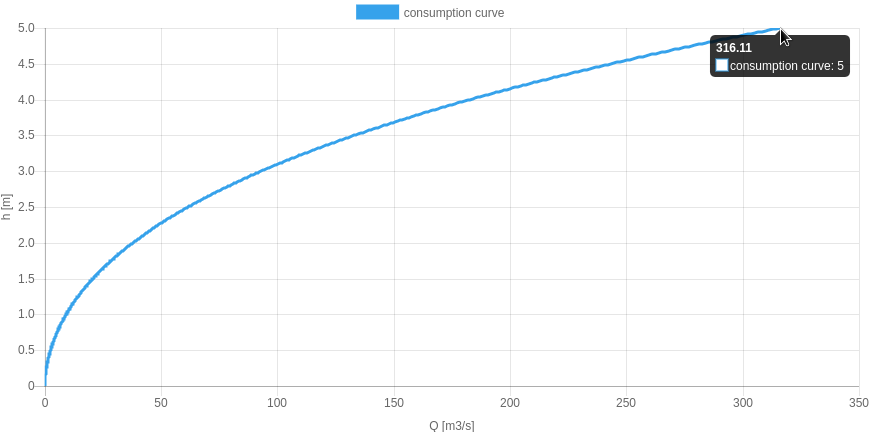
\includegraphics[width=\textwidth]{slike/izracuni/trapeznaMetoda_konsumpcijska.png}		
		\caption{Konsumpcijska krivulja izračunana po trapezni metodi}\label{fig:trapeznaMetoda_konsumpcijskaKrivulja}
	\end{centering}
\end{figure}



S slike~\ref{fig:trapeznaMetoda_konsumpcijskaKrivulja} lahko odčitamo pretok struge izračunane po trapezni metodi $Q(h=5m) = 316,1~m^3/s$. 


%-----------------------------------------------
\section{Izračun parametrov po numerični metodi}\label{sec:izracun_numericnaMetoda}

V tem poglavju bomo primerjali rezultate ročno izračunanih parametrov in parametrov izračunanih s programom po numerični metodi omenjeni v poglavju~\ref{sec:izracun_trapeznaMetoda}.


\subsection{Ročni izračun parametrov hidroelektrarne}\label{sec:izracun_rocno_numericnaMetoda}

\begin{enumerate}[I.]
	
	\item Odsek
	
	\begin{ceqn}
		\begin{align}
			S_I&=\dfrac{5  5}{2} = 12,5~m^2\\
			P_I&=\sqrt{5^2 + 5^2} = 7,07~m\\
			Q_I&=\dfrac{\sqrt{0,01}}{0,03} \cdot \dfrac{12,5^{5/3}}{7,07^{2/3}} = 60,9~m^3/s
		\end{align}
	\end{ceqn}
		
	\item Odsek
	
	\begin{ceqn}
		\begin{align}
			S_{II}&=55 = 25 ~m^2\\
			P_{II}&=5~m\\
			Q_{II}&=\dfrac{\sqrt{0,01}}{0,03} \cdot \dfrac{25^{5/3}}{5^{2/3}} = 243,7~m^3/s
		\end{align}
	\end{ceqn}
	
	\item Odsek
	\begin{ceqn}
		\begin{align}
		S_{III}&=S_{I} = 12,5~m^2\\
		P_{III}&=S_{I} = 7,07~m\\
		Q_{III}&=Q_{III} = 60,9~m^3/s
		\end{align}
	\end{ceqn}
	
\end{enumerate}

Skupni pretok za višino $h=5m$:

\begin{ceqn}
 \begin{align}
Q_{s} = Q_{I} + Q_{II} + Q_{III} = 60,9 + 243,7 + 60,9 = 365,5~m^3/s
 \end{align}
 \end{ceqn}




\subsection{Izračun parametrov hidroelektrarne s programom}

S pomočjo uporabniškega vmesnika v koordinatni sistem vnašamo serijo točk, s katerimi modeliramo robove izbrane struge. V tabeli na levi strani diagrama, za vsak odsek med dvema točkama dodajamo Manningove koeficiente hrapavosti $ng$ in naklone struge na sliki označene s $\varphi$. V našem primeru so vrednosti koeficientov za vse odseke rečne struge enake.

\begin{figure}[H]
	\begin{centering}
		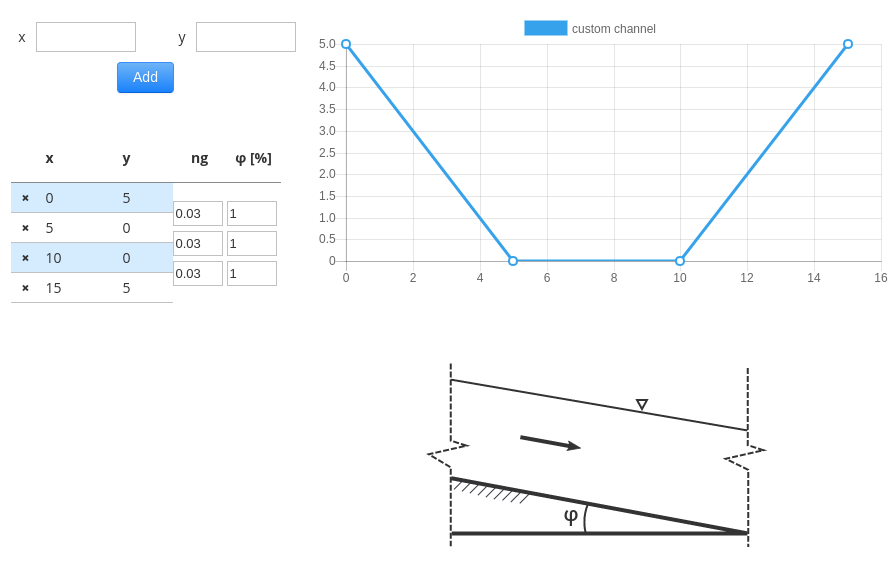
\includegraphics[width=\textwidth]{slike/izracuni/numericno_modeliranjeStruge.png}		
		\caption{Vnos podatkov v program}\label{fig:modeliranjeStruge}
	\end{centering}
\end{figure}

% H forces image to stand here on this place -> pushes text below
\begin{figure}[H]
	\begin{centering}
		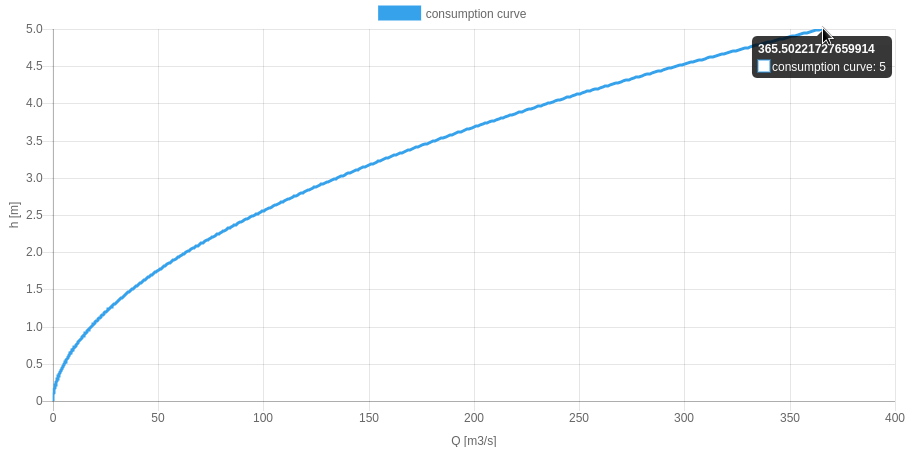
\includegraphics[width=\textwidth]{slike/izracuni/numericno_konsumpcijskaKrivulja.png}		
		\caption{Graf konsumpcijske krivulje izračunani po numerični metodi}\label{fig:custom_konsumpcijskaKrivulja}
	\end{centering}
\end{figure}


Z grafa konsumpcijske krivulje \ref{fig:custom_konsumpcijskaKrivulja} pri višini $h = 5m$ lahko preberemo da je pretok $Q=365,5~m^3/s$. Rezultat po numeričnem postopku izračunan s programom je enak rezultatu ki smo ga izračunali ročno v poglavju~\ref{sec:izracun_rocno_numericnaMetoda}




%----------------------------------------------
\section{Rezultati izračuna}
V poglavjih ~\ref{sec:izracun_trapeznaMetoda} in ~\ref{sec:izracun_numericnaMetoda} smo preverili da sta rezultata ročnega izračuna in izračuna s programom po enaki metodi enaka. Če primerjamo rezultate trapezne metode z rezultati numerične metode pa se rezultati razlikujejo. Razlog za to je v izbiri matematičnega modela, kar prikazujejo enačbe spodaj.

Primerjali bomo rezultata pretokov vodotoka po trapezni in numerični metodi. Pri tem uporabimo podatke iz naloge opisane v poglavju~\ref{sec:izracun}. Celotna površina prečnega prereza pod gladino vode $S(h)$ in omočeni obod struge $P(h)$ sta sestavljena iz treh odsekov kot je prikazano na sliki~\ref{fig:izracun_trapeznaStruga}. $Q_i$ predstavlja izračun pretoka po trapezni metodi, $Q_{ii}$ pa izračun pretoka po numerični metodi:
\begin{ceqn}
\begin{align}
S(h)&= S_I(h) + S_{II}(h) + S_{III}(h)\\
P(h)&= P_I(h) + P_{II}(h) + P_{III}(h)\\
Q_i &= \dfrac{\sqrt{I}}{ng} \cdot \dfrac{S^{5/3}}{P^{2/3}} \\
Q_{ii} &= \dfrac{\sqrt{I}}{ng} \cdot \dfrac{S_I^{5/3}}{P_I^{2/3}} + \dfrac{\sqrt{I}}{ng} \cdot \dfrac{S_{II}^{5/3}}{P_{II}^{2/3}} + \dfrac{\sqrt{I}}{ng} \cdot \dfrac{S_{III}^{5/3}}{P_{III}^{2/3}}
\end{align}
\end{ceqn}

Če v obeh enačbah odstranimo skupne člene enačbe, enačbe poenostavimo v:

\begin{ceqn}
\begin{align}
Q_i &=\dfrac{S^{5/3}}{P^{2/3}}\\
Q_{ii} &= \dfrac{S_I^{5/3}}{P_I^{2/3}} + \dfrac{S_{II}^{5/3}}{P_{II}^{2/3}} + \dfrac{S_{III}^{5/3}}{P_{III}^{2/3}}
\end{align}
\end{ceqn}


Enačimo obe enačbi in uporabimo podatke iz:
\begin{ceqn}
\begin{align}
Q_i &= Q_{ii}\\
\dfrac{S^{5/3}}{P^{2/3}} &= \dfrac{S_I^{5/3}}{P_I^{2/3}} + \dfrac{S_{II}^{5/3}}{P_{II}^{2/3}} + \dfrac{S_{III}^{5/3}}{P_{III}^{2/3}}\\
\dfrac{50^{5/3}}{19,14^{2/3}} &= \dfrac{12,5^{5/3}}{7,07^{2/3}} + \dfrac{25^{5/3}}{5^{2/3}} + \dfrac{12,5^{5/3}}{7,07^{2/3}}\\
94,84 &\neq 109,7
\end{align}
\end{ceqn}


Do razlike v rezultatih pride zaradi matematičnih pravil seštevanja potenc, kar smo pokazali z zgornjim izračunom:
\begin{ceqn}
\begin{align}
a^y + b^y \neq (a+b)^y
\end{align}
\end{ceqn}



